\documentclass[%
reprint,
amsmath,
amssymb,
aps]{revtex4-1}

\usepackage{graphicx}
\usepackage[mathletters]{ucs} % Extended unicode (utf-8) support
\usepackage[utf8x]{inputenc}
\usepackage{hyperref}
\usepackage{mhchem}

\begin{document}



\title{Development of a computer program for electronic structure calculation using Lagrange basis functions}
\author{Fadjar Fathurrahman, Hermawan K. Dipojono}
\affiliation{
Department of Engineering Physics, Bandung Institute of Technology \\
Research Center for Nanoscience and Nanotechnology, Bandung Institute of Technology
}

\begin{abstract}
Electronic structure calculation is one approach that can be used to study material,
especially at nanoscale where quantum nature of electrons might play important role
to determine material properties. Among various methods for electronic structure calculation,
density functional theory (DFT) based on Kohn-Sham equations is considered to be a popular one.
In the the implementation to solve Kohn-Sham equations, single-electron wave function must be
represented as an expansion of basis functions or some discretization schemes. Several
existing computer programs for DFT calculations, such as  Quantum Espresso and Gaussian09,
expand single-electron wave function using plane wave and Gaussian functions, respectively.
Others, such as Octopus and GPAW use discretization based on finite-difference scheme.
In this article, we report our initial effort to implement a new computer program to
solve Kohn-Sham equations using expansion in Lagrange basis functions (LFs).
Use of this basis set in Kohn-Sham equation results in matrix eigenproblem which
is similar to matrix eigenproblem in finite difference schemes. Two methods to solve
Kohn-Sham equation, namely self-consistent field iterations and direct minimization,
are reported. Comparisons done with finite difference scheme implemented in Octopus
for several simple systems shows that total energy convergence with respect to the number
of grid points is better when using Lagrange basis functions.
\end{abstract}

\maketitle

\section{Introduction}

Welcome to \ffrLFDFT documentation.
In this document you will find the following information:
\begin{itemize}
\item basic information about \ffrLFDFT
\item how to compile and use the program
\item implementation details of the program
\end{itemize}

{\tt ffr-LFDFT} is a poor man's program (or collection of subroutines, as of now)
to carry out electronic structure calculations based on density functional theory
and Lagrange basis set.

This program is intended for research in implementation of new methods in
electronic structure calculations in condensed matter.
Currently it is not as stable of functional
as more well-known package such as Quantum Espresso, ABINIT, or VASP.
However, it can be used to calculate total energy of solids.

This program is written mainly by me, Fadjar Fathurrahman at Research Center
of Nanoscience and Nanotechnology, Bandung Institute of Technology, Indonesia.


% Add tutorial on how to use m\_LF3d module to solve Schrodinger equation
% in 1d.
% In LF3d periodic, only gamma-point sampling is used.


\section{Theory}

\subsection{Kohn-Sham density functional theory}

Within LDA, Kohn-Sham energy functional can be written as \cite{Kohn1965}:
\begin{equation}
E_{\mathrm{LDA}}\left[\{\psi_{i}(\mathbf{r})\}\right] =
E_{\mathrm{kin}} + E_{\mathrm{ion}} + E_{\mathrm{Ha}} + E_{\mathrm{xc}}
\label{eq:KS_ene_func}
\end{equation}
with the following energy terms.
\begin{itemize}
\item Kinetic energy:
\begin{equation}
E_{\mathrm{kin}} = -\frac{1}{2}\sum_{i_{st}}
\int f_{i_{st}}
\psi_{i_{st}}^{*}(\mathbf{r})\,\nabla^2\,\psi_{i_{st}}(\mathbf{r})
\,\mathrm{d}\mathbf{r}
\end{equation}
%
\item ion-electron interaction energy:
\begin{equation}
E_{\mathrm{ion}} = \int V_{\mathrm{ion}}(\mathbf{r})\, \rho(\mathbf{r})\,
\mathrm{d}\mathbf{r}
\end{equation}
%
\item Hartree (electrostatic) energy:
\begin{equation}
E_{\mathrm{Ha}} = \int \frac{1}{2}
\dfrac{\rho(\mathbf{r})\rho(\mathbf{r}')}
{\left|\mathbf{r} - \mathbf{r}'\right|}
\mathrm{d}\mathbf{r}\mathrm{d}\mathbf{r}'
\end{equation}
%
\item Exchange-correlation energy (using LDA):
\begin{equation}
E_{\mathrm{xc}} = \int \epsilon_{\mathrm{xc}}\left[\rho(\mathbf{r})\right]
\rho(\mathbf{r})\,\mathrm{d}\mathbf{r}
\end{equation}
%
\end{itemize}

Application of variational principle to energy functional \ref{eq:KS_ene_func}
with the constraint
\begin{equation}
\int \psi^{*}_{i_{st}}(\mathbf{r}) \psi_{i_{st}}(\mathbf{r})\,\mathrm{d}\mathbf{r}
\end{equation}
results in the so-called Kohn-Sham equation:
\begin{equation}
\left[
-\frac{1}{2}\nabla^2  + V_{\mathrm{KS}}(\mathbf{r})
\right] \psi_{i_{st}}(\mathbf{r}) =
\epsilon_{i_{st}}\psi_{i_{st}}(\mathbf{r})
\end{equation}
where $\epsilon{i_{st}}$ and $\psi_{i_{st}}(\mathbf{r})$ is known as Kohn-Sham
eigenvalues and eigenvectors (orbitals).
Quantity $V_{\mathrm{KS}}$ is called the Kohn-Sham potential, which can be
written as sum of several potentials:
\begin{equation}
V_{\mathrm{KS}}(\mathbf{r}) = V_{\mathrm{ion}}(\mathbf{r}) + V_{\mathrm{Ha}}(\mathbf{r})
+ V_{\mathrm{xc}}(\mathbf{r})
\label{eq:KS-pot}
\end{equation}

$V_{\mathrm{ion}}$ denotes attractive potential between ion (or atomic nuclei)
with electrons. This potential can be written as:
\begin{equation}
V_{\mathrm{ion}}(\mathrm{r}) =
\sum_{I}^{N_{\mathrm{atoms}}}
\frac{Z_{I}}{ \left| \mathbf{r} - \mathbf{R}_{I} \right| }
\end{equation}
This potential is Coulombic and has singularities
at the ionic centers. It is generally difficult to describe this potential
numerically, so it is common to replace the full Coulombic potential
with softer potential which is known as pseudopotential.
There are various types or flavors of pseudopotentials.
In the current implementation, ion-electron potential, $V_{\mathrm{ion}}$
is treated by pseudopotential. HGH-type pseudopotential is employed due to the
the availability of analytic forms both in real and reciprocal space.

$V_{\mathrm{Ha}}$ is the classical Hartree potential. It is defined as
\begin{equation}
V_{\mathrm{Ha}}(\mathbf{r}) = \int
\frac{\rho(\mathbf{r}')}
{\mathbf{r} - \mathbf{r}'}\,\mathrm{d}\mathbf{r}',
\end{equation}
where $\rho(\mathbf{r})$ denotes electronic density:
\begin{equation}
\rho(\mathbf{r}) = \sum_{i_{st}=1}^{N_{\mathrm{occ}}}
f_{i_{st}}
\psi^{*}_{i_{st}}(\mathbf{r}) \psi_{i_{st}}(\mathbf{r})
\end{equation}
Alternatively, Hartree potential can also be obtained via solving Poisson equation:
\begin{equation}
\nabla^{2} V_{\mathrm{Ha}}(\mathbf{r}) = -4\pi \rho(\mathbf{r})
\end{equation}
The last term in Equation \eqref{eq:KS-pot} is exchange-correlation potential.

\subsection{Lagrange basis functions}

Use of Lagrange basis functions in electronic structure calculation is relatively new.
Familiy:

In this work, we will be using periodic Lagrange functions.

\begin{figure}
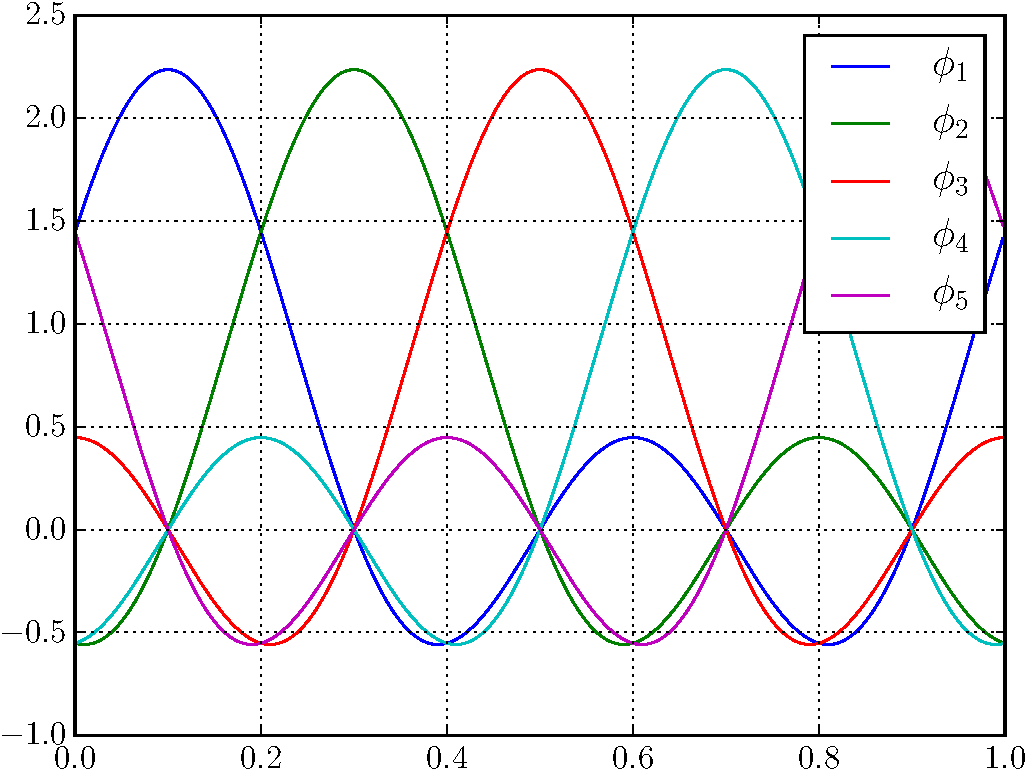
\includegraphics[width=0.5\textwidth]{images/plot_LF_p_N_5.pdf}
\end{figure}



\section{Implementation}

In this section, we wil describe our implementation of various terms 
in Kohn-Sham equations using Lagrange basis functions.
The computer program which contains our implementation can be found in public
repository: \url{https://github.com/f-fathurrahman/ffr-LFDFT}.

\subsection{Kohn-Sham equations in Lagrange basis functions representation}

Using Lagrange basis function \ref{eq:LF_p_1d} and its extension in 3d, Kohn-Sham orbitals
at point $\mathbf{r} = (x,y,z)$ can be written as
\begin{equation}
\psi_{i_{st}}(x,y,z) = \sum_{\alpha}^{N_x} \sum_{\beta}^{N_y} \sum_{\gamma}^{N_z}
C_{\alpha\beta\gamma}^{i_{st}} L_{\alpha}(x) L_{\beta}(y) L_{\gamma}(z)
\end{equation}
%
Using this expansion, kinetic operator can be written as
\begin{align}
T_{\alpha\beta\gamma}^{\alpha'\beta'\gamma'} & = -\frac{1}{2} \sum_{i_{st}} f_{i_{st}}
\Braket{ \psi_{i_{st}} | \nabla^2 | \psi_{i} } \\
& =
-\frac{1}{2}
\sum_{i_{st}} f_{i_{st}} \sum_{\alpha\alpha'} \sum_{\beta\beta'} \sum_{\gamma\gamma'}
C^{i_{st}}_{\alpha\beta\gamma} \mathbb{L}_{\alpha\beta\gamma}^{\alpha'\beta'\gamma'}
C^{i_{st}}_{\alpha'\beta'\gamma'}
\end{align}
%
were the Laplacian matrix $\mathbb{L}_{\alpha\beta\gamma}^{\alpha'\beta'\gamma'}$
has the following form:
\begin{equation}
\mathbb{L}_{\alpha\beta\gamma}^{\alpha'\beta'\gamma'} =
D^{(2)}_{\alpha\alpha'}\delta_{\beta\beta'}\delta_{\gamma\gamma'} +
D^{(2)}_{\beta\beta'}\delta_{\alpha\alpha'}\delta_{\gamma\gamma'} +
D^{(2)}_{\gamma\gamma'}\delta_{\alpha\alpha'}\delta_{\beta\beta'}
\end{equation}
%
Specifically, for periodic Lagrange basis function $D^{(2)}_{ij}$, $i, j = \alpha, \beta, \gamma$
can be written as follows.
\begin{equation}
D^{(2)}_{ij} = -\left( \frac{2\pi}{L} \right)^2 \frac{N'}{3} \left( N' + 1 \right) \delta_{ij} \\
+ \dfrac{ \left(\dfrac{2\pi}{L}\right)^2 (-1)^{i-j}\cos\left[\dfrac{\pi(i-j)}{N}\right]}
{2\sin^2\left[\dfrac{\pi(i-j)}{N}\right]}
(1-\delta_{nn'})
\label{eq:kin1d_p}
\end{equation}
where $N' = (N-1)/2$.

The matrix representation of kinetic operator is sparse.

The remaining potential terms which are local have very simple matrix form, i.e.
diagonal. The action of potential operator to Kohn-Sham orbital at point
$(r_{\alpha\beta\gamma})$ thus can be
obtained by pointwise multiplication with the potential on that point:
\begin{equation}
V_{\mathrm{KS}}(r_{\alpha\beta\gamma}) = V_{\mathrm{ion}}(r_{\alpha\beta\gamma}) +
V_{\mathrm{Ha}}(r_{\alpha\beta\gamma}) + V_{\mathrm{xc}}(r_{\alpha\beta\gamma})
\end{equation}

\subsection{Methods to solve Kohn-Sham equations}

We implement two methods to solve the Kohn-Sham equations, namely
via the self-consistent field (SCF) iterations and
direct energy minimization.

Outline of SCF iterations:
\begin{itemize}
\item Guess density $\rho(\mathbf{r})$
\item Iterate until convergence
\begin{itemize}
\item Calculate Kohn-Sham potentials $V_{\mathrm{KS}}$ and build the Kohn-Sham
Hamiltonian $H_{\mathrm{KS}}$
\item Diagonalize $H_{\mathrm{KS}}$ to obtain $\mathrm{\psi_{i_{st}}}(\mathbf{r})$
and $\epsilon_{i_{st}}$.
\item Calculate charge density and total energy. If the calculation converges
the stop the calculation, if not iterate.
\end{itemize}
\end{itemize}

Outline of direct minimization, using 
\begin{itemize}
\item Generate guess Kohn-Sham orbitals, orthonormalize if needed.
\item Calculate charge density, build Kohn-Sham potential and calculate total energy
for this
\item Iterate until convergence:
%
\begin{itemize}
%
\item Calculate Kohn-Sham electronic gradient $\mathbf{g}_{\psi}$ and the preconditioned
gradient $\mathbf{Kg}_{\psi}$ where $\mathbf{K}$ is a preconditioner.
%
\item Calculate search direction:
\begin{equation}
\beta = \dfrac{\mathbf{g}_{\psi}^{\dagger}\mathbf{Kg}_{\psi}}
{\mathbf{g}_{\psi,\mathrm{prev}}^{\dagger}\mathbf{Kg}_{\psi,\mathrm{prev}}}
\end{equation}
If $\mathbf{g}_{\psi,\mathrm{prev}}$ is not available (first iteration) then set
$\beta = 0$.
%
\item Calculate new direction:
\begin{equation}
\mathbf{d} = 
\end{equation}
\end{itemize}
%
\end{itemize}


\section{Numerical results}

\subsection{Gaussian potential}

To validate our implementation, we will calculate total energy of a system with
attractive "ionic" potential which has the following general form:
\begin{equation}
V_{\mathrm{ion}}(r) = -A\exp(-\alpha r^2)
\end{equation}
where $A$ and $\alpha$ are positive constants.
We compare the obtained electronic total energy using the one obtained by
\textsc{Octopus} program \cite{Marques2003,Castro2006,Xavier2015}
which implements finite difference approaches to solve Kohn-Sham equations.
 
The calculations are done using $16 \times 16 \times 16$ bohr periodic unit cell
and the center of the potential is set to be the center of the cell, i.e.
at coordinate $(8,8,8)$ bohr. The value of $A$ is set to 10 and we use 4 different
values of $\alpha$, i.e. 0.5, 1.0, 2.0, and 3.0. The visualization of the potential
is shown in Figure \ref{fig:gauss_pot}. Notice that the potential becomes sharper
as value of $\alpha$ becomes larger.
\begin{figure}
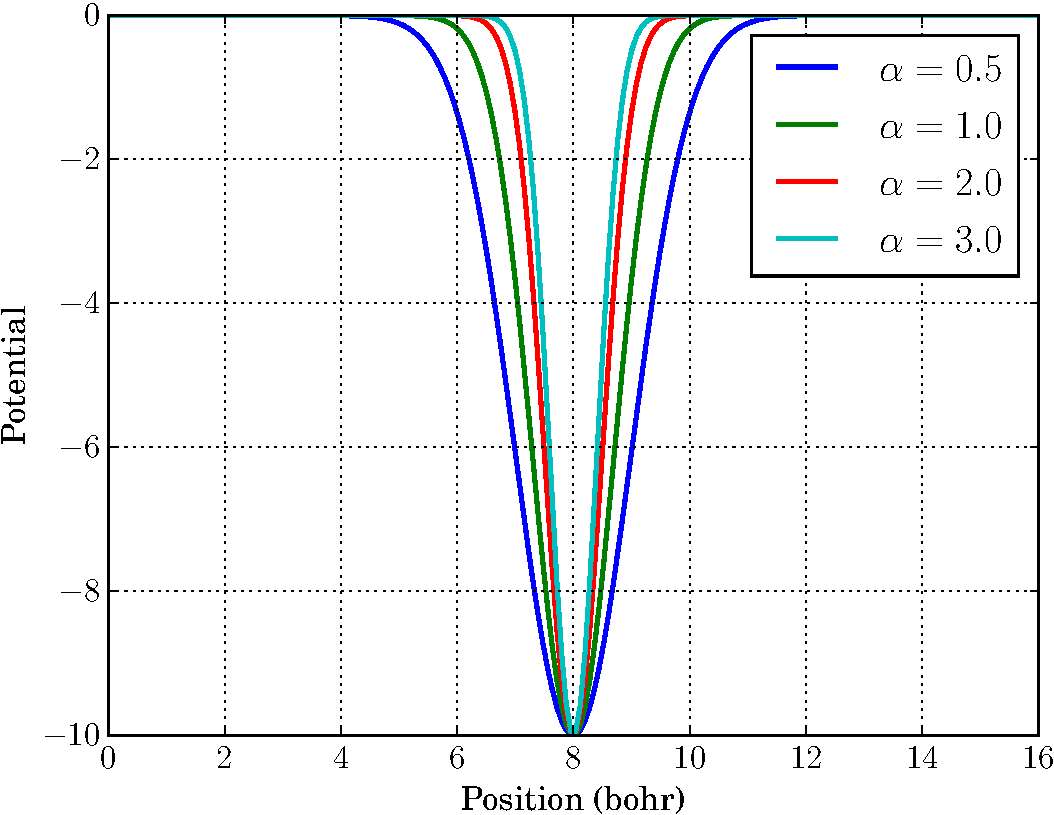
\includegraphics[width=0.5\textwidth]{images/V_gauss.pdf}
\caption{Gaussian potential}
\label{fig:gauss_pot}
\end{figure}

Result for Gaussian potential

\begin{figure*}[h]
\centering
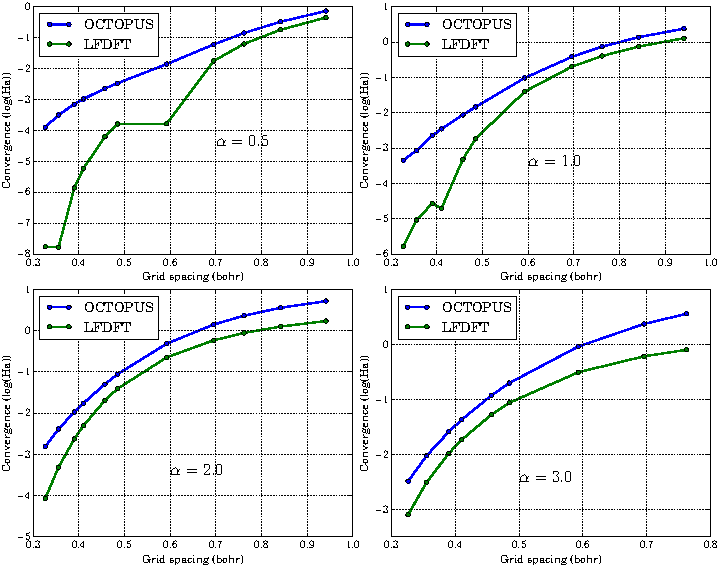
\includegraphics[scale=1.0]{images/COMBINE_v1.pdf}
\caption{Convergence}
\end{figure*}

Comparison between SCF and direct minimization:

\subsection{Hydrogen pseudopotential}

Result for atomic system

\begin{figure}
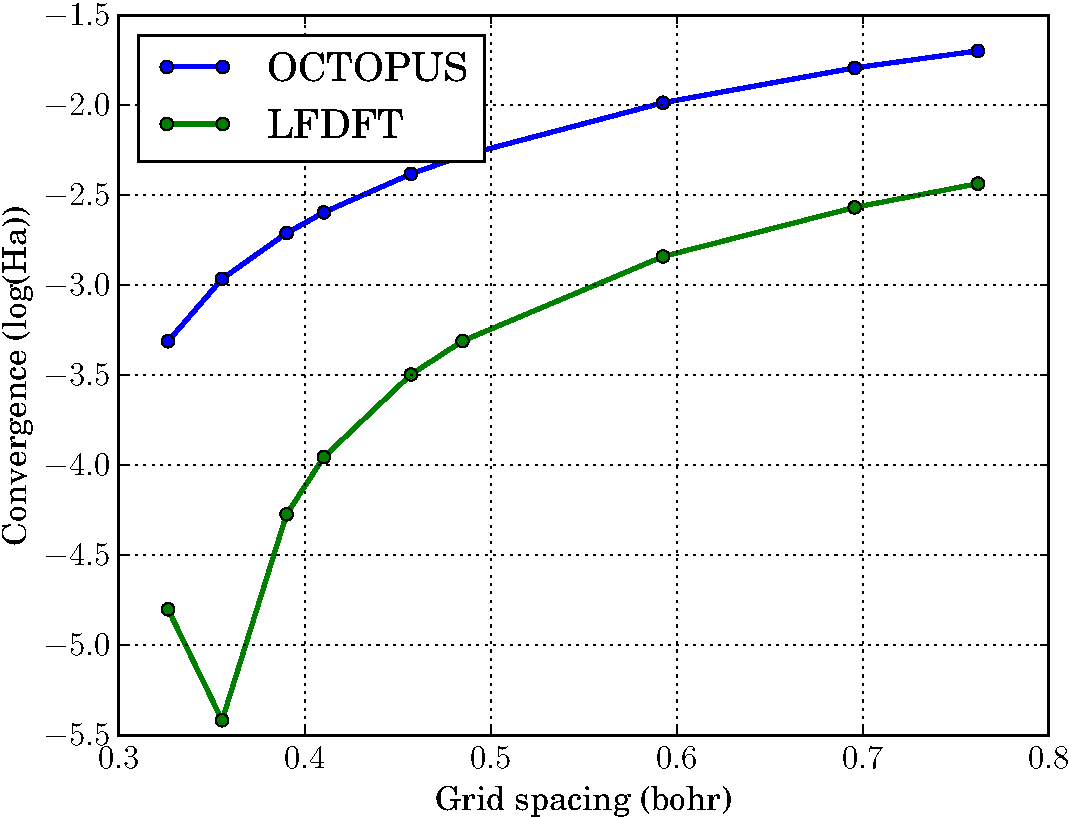
\includegraphics[width=0.5\textwidth]{images/CONV_atom_H.pdf}
\end{figure}

\subsection{Lithium pseudopotential}
Blah




\bibliography{LFDFT-v2}

\end{document}


